\documentclass[12pt,a4paper]{article}
\usepackage{graphicx}
\usepackage{wrapfig}
\usepackage{textcomp}

\title{Praktikum Physik - Leitercharakteristiken}
\author{Simon Marti, Patricia Schwab, Mirco Kocher}
\date{20.04.2012}


\begin{document}
\maketitle

\section*{Ziel}
Kennlinien verschiedener Elementen aufnehmen und auf Abweichungen vom ohmschen Gesetz untersuchen.

\section*{Motivation}
Der Versuch der Leitercharakteristiken eignet sich gut als Einstieg in die Elektronik. Dabei wird das Verhalten von h\"aufig verwendeten Bauteilen (Metalle, Halbleiter) in einem Stromkreis untersucht und deren jeweiligen charakteristischen Eigenschaften analysiert. Durch die herausragende Bedeutung der Halbleiter in der Elektronik werden sie in diesem Versuch besonders ber\"ucksichtigt.

\section*{Theorie}
Das ohmsche Gesetz ist durch foldende Formel definiert:
\begin{equation}
U=R\cdot I [\mbox{V}]
\end{equation}
wobei $U$ die Spannung, $R$ der Widerstand und $I$ die Stromst\"arke ist. 


Mit zunehmender Spannung (zunehmender Temperatur) nimmt beim Me-tall der Widerstand zu, da die Bewegung der Elektronen durch die verst\"arkte thermische Bewegung (Abnahme der mittleren freien Flugzeit) behindert wird.
Der Widerstand des Halbleiters nimmt bei zunehmender Spannung (zunehmender Temperatur) ab, da bei h\"oherer Temperatur mehr Ladungstr\"ager am Transport teilnehmen.
Beim ohmschen Widerstand ist das Verh\"altnis von Spannung zu Stromst\"arke linear.

\section*{Experiment}

\subsection*{Aufbau und Ablauf}
\begin{wrapfigure}{r}{8cm}
\vspace{-15pt}
\centering
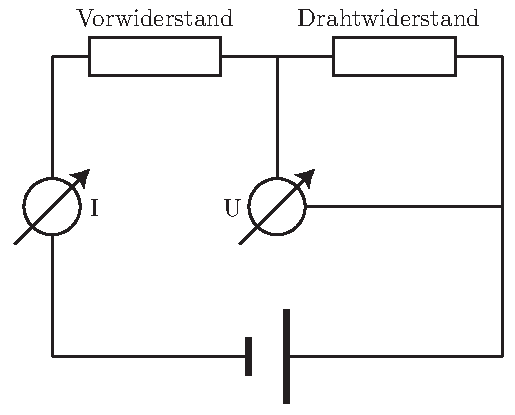
\includegraphics[width=6cm]{illustration.pdf}
\end{wrapfigure}
Um die Kennlinie verschiedener Elemente zu bestimmen werden diese gem\"ass dem Schaltschema rechts mit einer Stromquelle und zwei Messger\"aten verbunden. Je nach Element wird zus\"atzlich ein Vorwiderstand dazugeschaltet um das Element nicht zu \"uberlasten. Die Spannung wird nun schrittweise von Patricia erh\"oht und die Stromst\"arke und Spannung jeweils von Simon abgelesen. 


\subsection*{Rohdaten}
$s_U$ = 0.07V

\noindent
$s_I$ = 0.01$\mu$A

\subsubsection*{Drahtwiderstand 15$k\Omega$}
\begin{tabular}{|r|r|r|r|r|r|}
\hline
$U$ [V]&$I [\mu $A]&$U$ [V]&$I [\mu $A]&$U$ [V]&$I [\mu $A]\\
\hline
11.15&0.759&139.6&9.448&-80.2&-5.444\\
19.76&1.350&160.9&10.865&-100.4&-6.800\\
30.99&2.098&179.9&12.142&-119.0&-8.056\\
40.5&2.754&199.8&13.475&-140.3&-9.491\\
49.9&3.380&220.1&14.82&-160.3&-10.846\\
59.9&4.065&239.0&16.065&-180.4&-12.187\\
80.1&5.427&-21.9&-1.48&-200.3&-13.518\\
99.9&6.762&-39.3&-2.659&-220.9&-14.878\\
120.1&8.125&-61.3&-4.152&-238.5&-16.077\\
\hline
\end{tabular}

\subsubsection*{Metallfadenlampe 10$W$}
\begin{tabular}{|r|r|r|r|r|r|}
\hline
$U$ [V]&$I [\mu $A]&$U$ [V]&$I [\mu $A]&$U$ [V]&$I [\mu $A]\\
\hline
19.38&9.535&180.5&37.02&-159.5&-34.36\\
39.5&14.798&199.9&39.39&-139.0&-31.71\\
60.8&19.254&221.1&41.74&-120.0&-29.01\\
80.1&22.763&239.5&43.75&-100.6&-26.109\\
99.4&25.939&-239.5&-43.72&-80.7&-22.832\\
120.5&29.11&-219.1&-41.51&-59.6&-19.023\\
140.4&31.94&-199.8&-39.3&-41.5&-15.283\\
160.5&34.54&-180.8&-37.02&-19.86&-9.651\\
\hline
\end{tabular}

\subsubsection*{Kohlenfadenlampe 35$W$}
\begin{tabular}{|r|r|r|r|r|r|}
\hline
$U$ [V]&$I [\mu $A]&$U$ [V]&$I [\mu $A]&$U$ [V]&$I [\mu $A]\\
\hline
20.7&14.032&179.5&170.75&-120.7&-104.09\\
39.9&28.645&202.2&198.95&-99.5&-82.34\\
59.3&44.95&210.2&209.06&-80.4&-63.95\\
80.4&63.97&-210.4&-203.9&-60.9&-46.00\\
99.0&81.97&-199.5&-195.51&-40.4&-31.00\\
119.8&103.2&-179.8&-171.05&-20.25&-29.06\\
140.0&124.88&-160.8&-148.5&&\\
159.5&147.05&-139.5&-124.31&&\\
\hline
\end{tabular}

\subsubsection*{Silizium-Diode max 400$V$}
\begin{tabular}{|r|r|r|r|r|r|}
\hline
$U$ [V]&$I [\mu $A]&$U$ [V]&$I [\mu $A]&$U$ [V]&$I [\mu $A]\\
\hline
-19.65&-1.95&-139.1&-13.94&0.771&206500\\
-40.4&-4.06&-161.0&-16.12&0.749&119400\\
-59.2&-5.94&-180.7&-18.0&0.694&31000\\
-81.0&-8.12&-200.3&-20.09&0.635&7700\\
-99.8&-10.01&-221.2&-22.15&&\\
-120.2&-12.01&-2339.5&-23.98&&\\
\hline
\end{tabular}

\subsubsection*{Zenerdiode}
\begin{tabular}{|r|r|r|r|r|r|}
\hline
$U$ [V]&$I [\mu $A]&$U$ [V]&$I [\mu $A]&$U$ [V]&$I [\mu $A]\\
\hline
20.5&2.02&160.0&15.99&187.0&18.69\\
41.2&4.13&180.8&18.08&187.7&18.77\\
60.8&6.08&196.2&4843&188.3&55.00\\
80.0&7.98&188.9&170&-0.693&-20690\\
99.9&10.03&189.1&385&-0.668&-12894\\
120.7&12.06&189.4&504&-0.620&-3655\\
140.1&14.0&185.2&18.5&&\\
\hline
\end{tabular}

\subsubsection*{Glimmstabilisato 87$V$ max 60$mA$}
\begin{tabular}{|r|r|r|r|r|r|}
\hline
$U$ [V]&$I [\mu $A]&$U$ [V]&$I [\mu $A]&$U$ [V]&$I [\mu $A]\\
\hline
19.98&1.97&99.7&9.95&89.9&40260\\
40.7&4.09&88.8&4.34&90.4&49030\\
60.9&6.09&92.7&13747&91.2&56750\\
79.3&7.92&89.0&28943&&\\
\hline
\end{tabular}

\subsection*{Auswertung}
Die Fehlerbalken wurden weggelassen, da sie kleiner als die Messpunkte selbst w\"aren.

\subsubsection*{Drahtwiderstand}
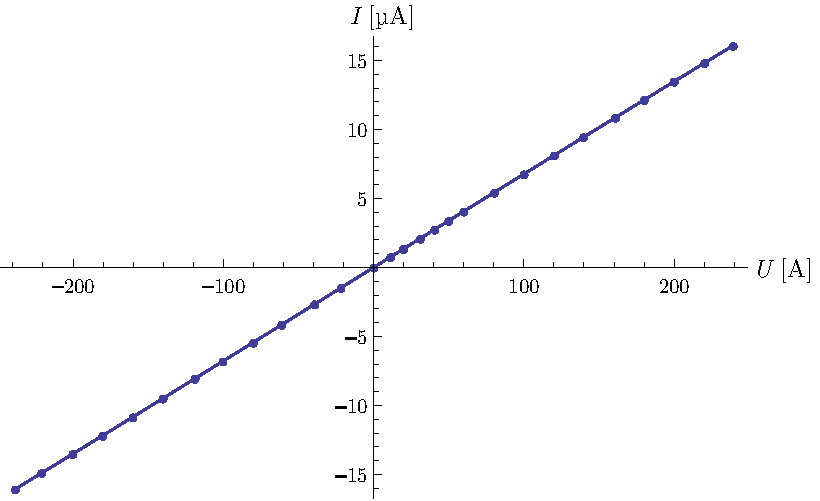
\includegraphics[width=14cm]{draht.pdf}
Mit linearer Interpolation.

\subsubsection*{Metallfadenlampe}
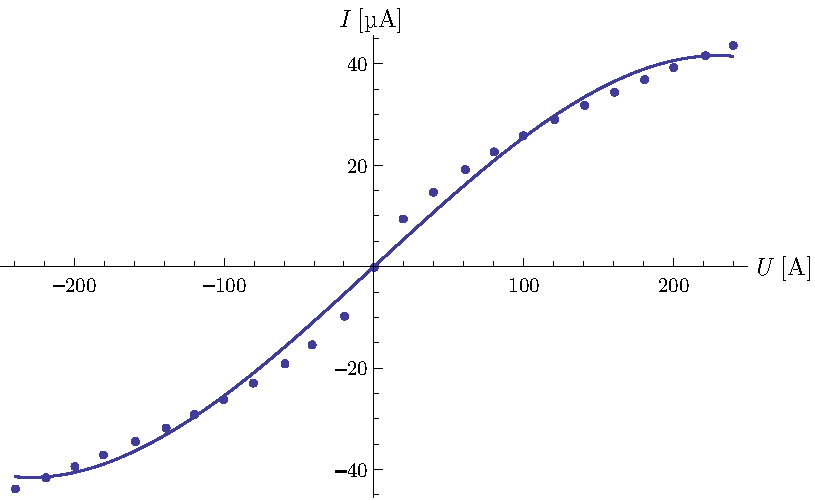
\includegraphics[width=14cm]{metallfadenlampe.pdf}
Mit kubischer Interpolation.

\subsubsection*{Kohlenfadenlampe}
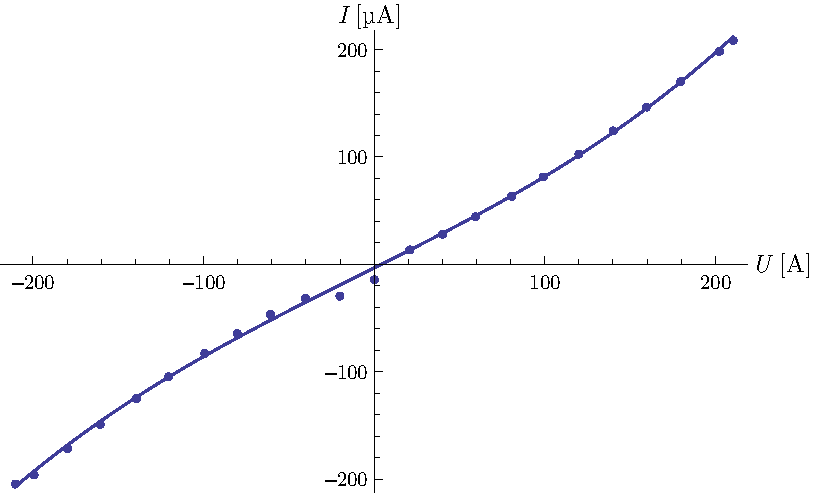
\includegraphics[width=14cm]{kohlenfadenlampe.pdf}
Mit kubischer Interpolation.

\subsubsection*{Silizium-Diode}
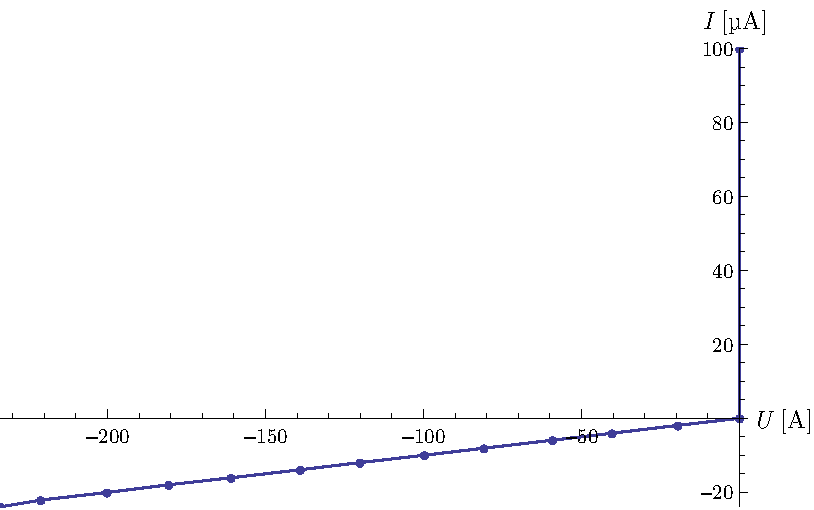
\includegraphics[width=14cm]{siliziumdiode.pdf}

\subsubsection*{Zenerdiode}
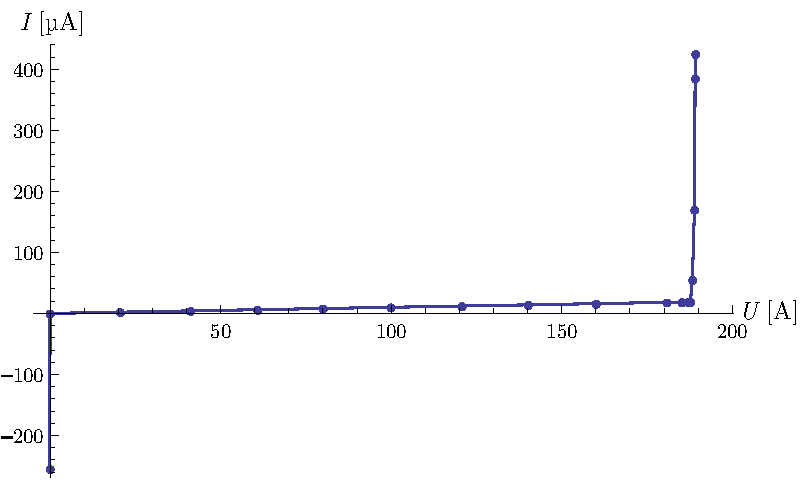
\includegraphics[width=14cm]{zenerdiode.pdf}

\subsubsection*{Glimmstabilisator}
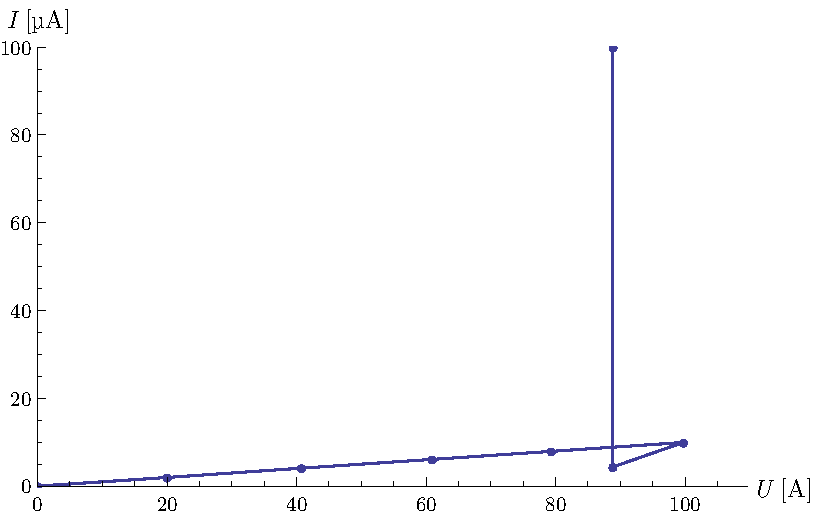
\includegraphics[width=14cm]{glimmstabilisator.pdf}


\subsection*{Diskussion}
Der Drahtwiderstand geh\"ort zu den ohmschen Widerst\"anden. Die Metallfadenlampe ist ein Metallleiter.
Als Halbleiter bezeichnet man die Kohlenfadenlampe, die Siliziumdiode, die Zenerdiode und den Glimmstabilisator.

Die Silizium-Diode und die Zenerdiode funktioniert nur in eine Richtung, deshalb sind die Messpunkte in Sperrrichutung jeweils nahe bei $0$. 

Beim Glimmstabilisator ist die Kennlinie solange linear bis er gl\"uht. Danach wird die Spannung nicht mehr h\"oher als die vorgesehenen 87$V$.

\subsection*{Aufgabe 3}
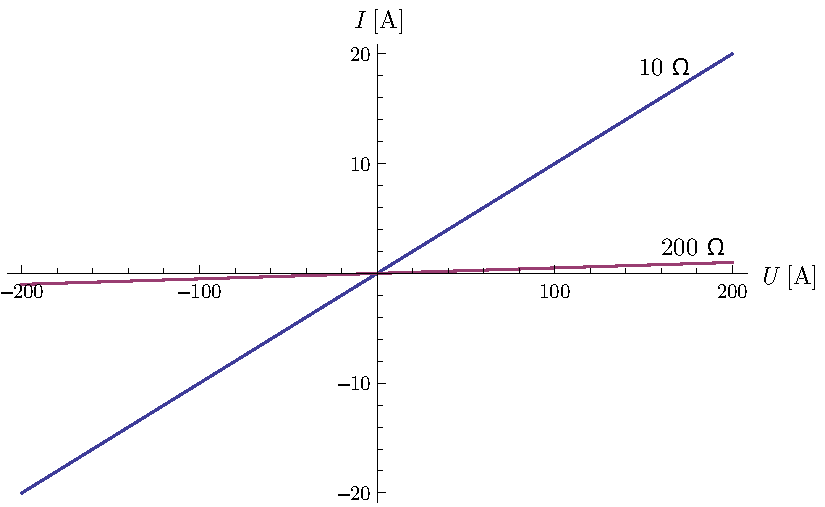
\includegraphics[width=15cm]{ohm.pdf}

Die Kennlinie wird immer steiler, je kleiner der Widerstand ist. Das ohmsche Gesetz sagt, dass $\frac{1}{R}$ die Steigung der Kennlinie ist. Wenn der Widerstand gegen $0$ geht, so wird die Steigung $\infty$. Deshalb ist die Kennlinie f\"ur einen idealen Leiter senkrecht.

\newpage
\section*{Theorieaufgaben}

\subsection*{Aufgabe 2}
\subsubsection*{Knotenregel}
Die Summe der zu- und wegfliessenden Str\"omen in einem Knoten ist Null, d.h.
\[ \sum_kI_k = 0 \]
Die Knotenregel folgt aus der Ladungserhaltung.

\subsubsection*{Maschenregel}
Die Summe aller Spannungsabf\"alle an den einzelnen Elementen, aus denen eine Masche besteht, ist Null, d.h.
\[ \sum_kU_k = 0\]
Die Maschenregel folgt aus der Energieerhaltung.

\subsection*{Aufgabe 3}
\begin{wrapfigure}{r}{8cm}
\centering
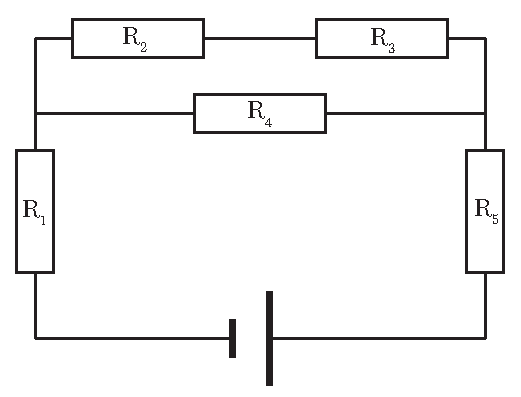
\includegraphics[width=6cm]{exercise3.pdf}
\end{wrapfigure}
\begin{eqnarray*}
R & = & \frac{38}{g} k\Omega \\
I & = & \frac{U}{R} = \frac{9}{38000} \cdot U_0
\end{eqnarray*}

Aus der Knotenregel
\begin{eqnarray*}
I_5 & = & I_{23} + I_4 \hspace{20pt} ( I_{23} = I_2 = I_3 ) \\
I_1 & = & I_3 + I_4 \hspace{20pt} ( I = I_1 = I_5 )
\end{eqnarray*}
folgt:
\begin{eqnarray*}
U_5 & = & I \cdot R_5 = \frac{9}{38000} \cdot U_0 \cdot 10^3 = \frac{9}{38} \cdot U_0 = I \cdot R_1 = U_1 \\
I_{23} & = & \frac{U_5}{R_{23}} = \frac{9}{38} \cdot U_0 \cdot \frac{1}{5000} = I_2 = I_3 \\
\Rightarrow & U_2 & = R_2 \cdot I_2 = \frac{9}{38} \cdot \frac{2000}{5000} \cdot U_0 = \frac{9}{95} \cdot U_0 \\
& U_3 & = R_3 \cdot I_3 = \frac{9}{38} \cdot \frac{3000}{5000} \cdot U_0 = \frac{27}{190} \cdot U_0 \\
I_4 & = & \frac{U_5}{R_4} \\
U_4 & = & I_4 \cdot R_4 = \frac{U_5}{R_4} = U_5 = \frac{9}{38} \cdot U_0
\end{eqnarray*}
\"Uberpr\"ufung:
\[ \sum_{i=1}^5 U_i = 3 \cdot \frac{9}{38} \cdot U_0 + \frac{9}{95} \cdot U_0 = U_0 \]

\subsection*{Aufgabe 5}
$R_i = 1\Omega$, Messbereich 0-1A, gew\"unschter Bereich 0-10A
\begin{eqnarray*}
I_n & = & 10 - 1 = 9\mbox{A (Strom durch den Nebenwiderstand)} \\
R_n & = & \frac{U_{max}}{I_n} = \frac{1}{9}  \Omega
\end{eqnarray*}
$R_n$ muss parallel geschaltet werden.
\begin{eqnarray*}
R_{Ges} & = & \left( \frac{1}{R_i} + \frac{1}{R_n} \right) ^{-1} = \frac{1}{10}\Omega \\
R_{Ges} \cdot I & = & U_{max} \\
\frac{1}{10} \cdot 10 & = & 1 \mbox{V}
\end{eqnarray*}

\end{document}